% Copyright 2026 Sreeram Anil
% SPDX-License-Identifier: CC-BY-4.0
% =============================================================================
%  Mahony explicit complementary filter on SO(3) — attitude (AHRS) family
% =============================================================================
\chapter{Explicit Complementary Filter on \texorpdfstring{$SO(3)$}{SO(3)} (Mahony)}
\label{ch:att-mahony}

\section*{At a glance}
\begin{tabular}{@{}l>{\raggedright\arraybackslash}p{0.76\textwidth}@{}}
Family & attitude / AHRS \\
Header & \texttt{include/estkit/attitude/mahony.hpp} \\
Registered names & \texttt{Mahony} (published), \texttt{Mahony-Gated} (practical variant) \\
State & unit quaternion $\bm{q}\in S^3$ and gyro bias $\bm{b}\in\real^3$ (7 reals) \\
Cost per step & $\approx150$ flops, one $\exp$;
  $130$ / $\SI{132}{\nano\second}$ per step, 312\,bytes \\
Tuning & $k_P=1\,\SI{}{\per\second}$, $k_I=0.1\,\SI{}{\per\second\squared}$, $k_a=k_m=1$ \\
Primary references & \cite{mahony2008,hamel2006,euston2008} \\
\end{tabular}

\section{Motivation and aerospace relevance}
The complementary filter of Chapter~\ref{ch:att-complementary} reconstructs an attitude from the
vector observations and then blends two attitudes. Mahony, Hamel and Pflimlin~\cite{mahony2008}
observed that the reconstruction step is unnecessary and, worse, ill-conditioned: what the sensors
actually deliver are \emph{directions}, and directions can be compared directly on $SO(3)$ by a
cross product. Their ``explicit complementary filter'' feeds the weighted sum of those cross
products back as a rate correction, adds an integrator to absorb the gyro bias, and propagates the
estimate with the corrected rate. The result is an observer with a global (more precisely,
almost-global) stability proof, no trigonometry, no matrix inversion and no singularity anywhere.

Two properties make it the standard nonlinear attitude observer in robotics and UAV autopilots.
First, it is \emph{passive}: the innovation term enters as a torque-like feedback and the Lyapunov
argument reduces to a dissipation inequality, so stability does not depend on linearisation.
Second, the bias integrator provides exactly the state that the fixed-gain complementary filter
lacks, at a cost of three extra reals, which removes the $b\tau$ steady-state error
(\eqref{eq:cf-bias}).

The same group's fixed-wing paper~\cite{euston2008} --- the centripetal correction of
Chapter~\ref{ch:att-complementary} --- is the acknowledgement that the observer's assumption
``the accelerometer measures gravity'' is the one thing the proof cannot repair.

\section{Problem statement and assumptions}
Conventions as in Chapter~\ref{ch:att-complementary}. Let $\{\bm{v}_{0i}\}_{i=1}^{n}$ be known unit
directions in the NAV frame and $\bm{v}_i$ their measured BODY counterparts,
\begin{equation}
\bm{v}_i = \bm{R}^\T\bm{v}_{0i} + \text{noise} .
\label{eq:mh-obs}
\end{equation}
Here $n=2$: $\bm{v}_{01}=[0,0,-1]^\T$ with $\bm{v}_1=\bm{f}/\norm{\bm{f}}$, and
$\bm{v}_{02}=\bm{m}_{\text{nav}}/\norm{\bm{m}_{\text{nav}}}$ with $\bm{v}_2=\bm{m}/\norm{\bm{m}}$.
The gyro model is $\bm{\omega}_y=\bm{\omega}+\bm{b}+\bm{n}_v$ with $\bm{b}$ constant or slowly
varying. The filter estimates $(\bm{q},\bm{b})$ and makes no stochastic assumption: it is an
observer, and the gains are chosen by pole placement on the linearised error dynamics rather than
by a Riccati equation.

\section{Derivation}

\subsection{The innovation}
Define the weighted sum of cross products between measured and predicted directions
(Mahony et al.~\cite{mahony2008}, Eq.~(32a)):
\begin{equation}
\hat{\bm{v}}_i = \bm{R}(\hat{\bm{q}})^\T\bm{v}_{0i},
\qquad
\bm{\omega}_{\text{mes}} = \sum_{i=1}^{n} k_i\,\big(\bm{v}_i\times\hat{\bm{v}}_i\big)\ \in\real^3 .
\label{eq:mh-wmes}
\end{equation}
Write the true attitude multiplicatively as $\bm{q}=\hat{\bm{q}}\otimes\exp(\bm{\delta})$ with
$\bm{\delta}\in\real^3$ a BODY-frame rotation vector. Then
$\bm{R}^\T = \exp(-[\bm{\delta}]_\times)\hat{\bm{R}}^\T$ and, to first order,
$\bm{v}_i = \hat{\bm{v}}_i-\bm{\delta}\times\hat{\bm{v}}_i$, so
\begin{align}
\bm{v}_i\times\hat{\bm{v}}_i
 &= -\big(\bm{\delta}\times\hat{\bm{v}}_i\big)\times\hat{\bm{v}}_i + O(\norm{\bm{\delta}}^2)
  = \big(\bm{I}-\hat{\bm{v}}_i\hat{\bm{v}}_i^\T\big)\bm{\delta} + O(\norm{\bm{\delta}}^2),\nonumber\\
\bm{\omega}_{\text{mes}} &= \bm{M}\,\bm{\delta} + O(\norm{\bm{\delta}}^2),
\qquad
\bm{M} := \sum_i k_i\big(\bm{I}-\hat{\bm{v}}_i\hat{\bm{v}}_i^\T\big) = \bm{M}^\T\succeq0 .
\label{eq:mh-lin}
\end{align}
$\bm{M}$ is positive \emph{definite} as soon as two of the $\hat{\bm{v}}_i$ are non-collinear: each
term annihilates only the direction $\hat{\bm{v}}_i$ itself, so the intersection of the null spaces
is empty. That is precisely the observability condition for two-vector attitude determination, and
it fails --- with visible consequences, see Chapter~\ref{ch:att-triad} --- when gravity and the
magnetic field are measured nearly parallel.

\subsection{The filter}
The explicit complementary filter with bias estimation is (\cite{mahony2008}, Eqs.~(32)--(33))
\begin{align}
\dot{\hat{\bm{R}}} &= \hat{\bm{R}}\,\big[\bm{\omega}_y-\hat{\bm{b}}+k_P\,\bm{\omega}_{\text{mes}}\big]_\times ,
 \label{eq:mh-R}\\
\dot{\hat{\bm{b}}} &= -k_I\,\bm{\omega}_{\text{mes}} ,
 \label{eq:mh-b}
\end{align}
with $k_P,k_I>0$. In quaternion form the propagation is the exact exponential map, so the unit norm
is preserved by construction,
\begin{equation}
\hat{\bm{q}}_{k+1} = \hat{\bm{q}}_k\otimes\exp\!\big(\bm{\omega}_c\dt\big),
\qquad \bm{\omega}_c = \bm{\omega}_y-\hat{\bm{b}}+k_P\bm{\omega}_{\text{mes}} .
\label{eq:mh-prop}
\end{equation}

\subsection{Why these signs, and the closed loop}
With $\tilde{\bm{b}}=\bm{b}-\hat{\bm{b}}$ and the noise dropped,
$\bm{\omega}_c = \bm{\omega}+\tilde{\bm{b}}+k_P\bm{\omega}_{\text{mes}}$. Differentiating
$\exp(\bm{\delta})=\hat{\bm{q}}^*\otimes\bm{q}$ and keeping first-order terms,
\begin{equation}
\dot{\bm{\delta}} = \bm{\omega}-\bm{\omega}_c = -k_P\bm{\omega}_{\text{mes}} - \tilde{\bm{b}},
\qquad
\dot{\tilde{\bm{b}}} = -\dot{\hat{\bm{b}}} = +k_I\bm{\omega}_{\text{mes}} .
\label{eq:mh-err}
\end{equation}
Substituting \eqref{eq:mh-lin} gives the linear error system
\begin{equation}
\begin{bmatrix}\dot{\bm{\delta}}\\ \dot{\tilde{\bm{b}}}\end{bmatrix}
=\begin{bmatrix}-k_P\bm{M} & -\bm{I}\\ k_I\bm{M} & \bm{0}\end{bmatrix}
\begin{bmatrix}\bm{\delta}\\ \tilde{\bm{b}}\end{bmatrix},
\qquad\text{characteristic polynomial}\quad
s^2 + k_P\mu\,s + k_I\mu = 0
\label{eq:mh-poly}
\end{equation}
for each eigenvalue $\mu>0$ of $\bm{M}$: a second-order loop with
$\omega_n=\sqrt{k_I\mu}$ and damping $\varsigma = \tfrac12 k_P\sqrt{\mu/k_I}$. The unique
equilibrium is $\bm{\delta}=\bm{0},\ \tilde{\bm{b}}=\bm{0}$, so the observer estimates the bias
correctly --- which the fixed-gain filter of Chapter~\ref{ch:att-complementary}, with
$k_I=0$, cannot. Note that the signs of \eqref{eq:mh-R}--\eqref{eq:mh-b} are not interchangeable:
$+k_P$ in the rate and $-k_I$ in the integrator are what make \eqref{eq:mh-poly} Hurwitz.

\subsection{Lyapunov / passivity argument}
The first-order analysis above is local. The contribution of \cite{mahony2008} is the global one.
With $\bm{E}=\bm{R}\hat{\bm{R}}^\T$ the NAV-frame attitude error and
$\bm{M}_0=\sum_i k_i\bm{v}_{0i}\bm{v}_{0i}^\T$, take
\begin{equation}
V = \sum_i k_i\big(1-\bm{v}_i^\T\hat{\bm{v}}_i\big) + \frac{1}{2k_I}\norm{\tilde{\bm{b}}}^2
  = \tr\!\big(\bm{M}_0(\bm{I}-\bm{E})\big) + \frac{1}{2k_I}\norm{\tilde{\bm{b}}}^2 \;\ge 0 ,
\label{eq:mh-V}
\end{equation}
which vanishes only at $\bm{E}=\bm{I}$, $\tilde{\bm{b}}=\bm{0}$ when $\bm{M}_0$ has full rank.
Differentiating along \eqref{eq:mh-R}--\eqref{eq:mh-b}, the bias terms cancel between the two
channels --- this is the passivity structure: the attitude error supplies
$\bm{\omega}_{\text{mes}}$ to the integrator and the integrator returns $-\tilde{\bm{b}}$ to the
attitude channel through a skew interconnection --- and there remains
\begin{equation}
\dot V = -k_P\,\norm{\bm{\omega}_{\text{mes}}}^2 \;\le\;0 .
\label{eq:mh-Vdot}
\end{equation}
LaSalle's invariance principle applied to \eqref{eq:mh-Vdot} shows that all trajectories converge to
the set $\{\bm{\omega}_{\text{mes}}=\bm{0}\}$, on which $\tilde{\bm{b}}\to\bm{0}$ as well; the
desired equilibrium is locally exponentially stable and the remaining equilibria (rotations by
$\pi$ about the eigenvectors of $\bm{M}_0$) are unstable and form a set of measure zero. This is
Theorem~5.1 of \cite{mahony2008}: \emph{almost-global} asymptotic stability, the strongest result
available on a compact manifold, where global asymptotic stability by a continuous feedback is
topologically impossible.

\subsection{Two optional refinements}
The implementation offers, both off by default:
\emph{(i)} \code{mag\_yaw\_only} --- project $\bm{v}_2\times\hat{\bm{v}}_2$ onto the body-frame
vertical $\hat{\bm{R}}^\T\bm{e}_3$ so that the magnetometer cannot influence roll and pitch;
\emph{(ii)} \code{mag\_ref\_measured} --- rebuild $\bm{v}_{02}$ from the measurement in Madgwick's
way \eqref{eq:mw-flux} instead of using the known field. Both cost accuracy here (results below):
with a \emph{known} reference the magnetometer is a full 3-D observation and contributes to $\bm{M}$
in all directions, and throwing that information away is not free.

\code{mag\_ref\_measured} is nevertheless what \code{ahrs.filters.Mahony} implements, so it is the
setting used for the cross-validation: with it enabled the two implementations agree to
$0.0014^\circ$ maximum angular distance over the $9\times10^4$ samples of the nominal flight
(Table~\ref{tab:val_ahrs}), both scoring $\SI{22.64}{\degree}$ RMS --- against the
$\SI{18.40}{\degree}$ of the registered configuration, which uses the known reference as the 2008
paper does. The residual difference between the two codes is that estkit propagates with the exact
exponential map \eqref{eq:mh-prop} while \code{ahrs} takes an Euler step on $\dot{\bm{q}}$, an
$O(\dt^3)$ effect.

\section{Algorithm}
\begin{algorithm}[H]
\caption{Mahony explicit complementary filter --- one sampling period}
\begin{algorithmic}[1]
\Require $\hat{\bm{q}}_{k-1},\hat{\bm{b}}_{k-1},\bm{\omega}_y,\bm{f},\bm{m}$; $k_P,k_I,k_a,k_m$
\State $\hat{\bm{v}}_1\gets\bm{R}(\hat{\bm{q}})^\T[0,0,-1]^\T$;\;
       $\bm{\omega}_{\text{mes}}\gets k_a\,(\bm{f}/\norm{\bm{f}})\times\hat{\bm{v}}_1$
\State $\hat{\bm{v}}_2\gets\bm{R}(\hat{\bm{q}})^\T\hat{\bm{m}}_{\text{nav}}$;\;
       $\bm{\omega}_{\text{mes}}\mathrel{+}= k_m\,(\bm{m}/\norm{\bm{m}})\times\hat{\bm{v}}_2$
\State $\hat{\bm{b}}\gets\operatorname{clamp}\big(\hat{\bm{b}}-k_I\bm{\omega}_{\text{mes}}\dt\big)$
       \Comment{integrator, \eqref{eq:mh-b}}
\State $\bm{\omega}_c\gets\bm{\omega}_y-\hat{\bm{b}}+k_P\bm{\omega}_{\text{mes}}$
\State $\hat{\bm{q}}_k\gets\hat{\bm{q}}\otimes\exp(\bm{\omega}_c\dt)$, normalise
       \Comment{propagation, \eqref{eq:mh-prop}}
\Ensure $\hat{\bm{q}}_k,\hat{\bm{b}}_k$
\end{algorithmic}
\end{algorithm}

\section{Application to the benchmark flight}
$k_P=\SI{1}{\per\second}$ is the value the assignment prescribes and the one used in the paper's
experiments. With two unit direction measurements and $k_a=k_m=1$, $\bm{M}$ has eigenvalues near
unity, so \eqref{eq:mh-poly} gives $\omega_n=\sqrt{k_I}$ and $\varsigma=k_P/(2\sqrt{k_I})$.
$k_I=\SI{0.1}{\per\second\squared}$ --- the bottom of the assignment's $0.1$--$0.3$ band --- gives
$\omega_n=\SI{0.32}{\radian\per\second}$ and $\varsigma=1.6$: an over-damped attitude loop with a
$\SI{3}{\second}$ time constant and a bias loop of about $\SI{20}{\second}$. The same gains are used
for both registered instances.

$k_I$ was kept at the bottom of the band for a measured reason: the specific-force disturbance of
the coordinated turns drives $\bm{\omega}_{\text{mes}}$ with a long-lived non-zero mean, and the
integrator \eqref{eq:mh-b} converts that into bias error. On \texttt{nominal} the bias RMSE grows
$0.62\to1.25\to2.41\to\SI{2.63}{\degree\per\second}$ as $k_I$ goes $0\to0.1\to0.2\to0.3$, and the
attitude RMS grows with it ($11.97\to18.46\to30.03\to\SI{28.10}{\degree}$).

Everything else is the published algorithm: known inertial reference directions, equal weights, no
manoeuvre rejection.

\section{Implementation notes}
One step is two rotation-matrix--vector products ($2\times9$ MACs, the matrix itself
$\approx20$ flops), two cross products, one clamp and one quaternion exponential: about 150 flops
with a single $\sin/\cos$ pair. Measured $\SI{130}{\nano\second}$/step ($\SI{132}{\nano\second}$
for the gated instance); \code{sizeof} is 312\,bytes. This is the cheapest \emph{bias-estimating}
filter in the family, a factor of 15 below the MEKF.

Numerical hygiene: the quaternion is renormalised inside \code{Quat::integrate}; each branch is
skipped if its measurement magnitude is below $10^{-6}$; the bias state is clamped to
$\pm\SI{10}{\degree\per\second}$, which is the anti-windup that keeps the integrator bounded when the
accelerometer is disturbed for minutes at a time (without it the \texttt{gyro\_bias} run winds past
$\SI{20}{\degree\per\second}$). There is no covariance, hence nothing to keep positive definite, and
the single-precision build reproduces the double-precision mission RMS to four digits.

The limitation is the one the Lyapunov proof makes explicit: \eqref{eq:mh-Vdot} guarantees that the
filter converges to the attitude \emph{consistent with the measured directions}. If the measured
gravity direction is wrong by $23^\circ$ for $\SI{60}{\second}$, the observer converges, correctly
and provably, to the wrong attitude.

\section{Benchmark results}
% Copyright 2026 Sreeram Anil
% SPDX-License-Identifier: CC-BY-4.0
\begin{table}[H]\centering\footnotesize\setlength{\tabcolsep}{3.5pt}\caption{Mahony: attitude benchmark (mean over seeds; all angles in degrees; $t_\mathrm{conv}$: first time the attitude error stays below 2$^\circ$ for 30\,s; bias RMSE in deg/s; 312 bytes of state).}\label{tab:imu_Mahony}
\begin{tabular}{lrrrrrrrrcr}\toprule scenario & RMS & roll & pitch & yaw & max & RMS$_\mathrm{ss}$ & $t_\mathrm{conv}$ [s] & bias RMSE & lost & ns/step \\ \midrule
nominal & 18.40 & 6.24 & 2.94 & 17.30 & 76.3 & 19.33 & 24 & 1.24 & yes & 130 \\
init\_error & 18.51 & 6.28 & 2.98 & 17.41 & 76.3 & 19.33 & 70 & 1.28 & yes & 130 \\
gyro\_bias & 18.44 & 6.25 & 2.94 & 17.35 & 76.3 & 19.33 & 32 & 1.28 & yes & 130 \\
mag\_disturbance & 20.41 & 6.33 & 3.17 & 19.35 & 76.3 & 19.33 & 24 & 1.35 & yes & 130 \\
vibration & 18.28 & 6.23 & 2.95 & 17.17 & 75.6 & 19.25 & 71 & 1.23 & yes & 130 \\
high\_dynamics & 18.75 & 6.42 & 3.01 & 17.63 & 77.3 & 19.62 & -- & 1.26 & yes & 130 \\
\bottomrule\end{tabular}\end{table}

\begin{figure}[H]\centering
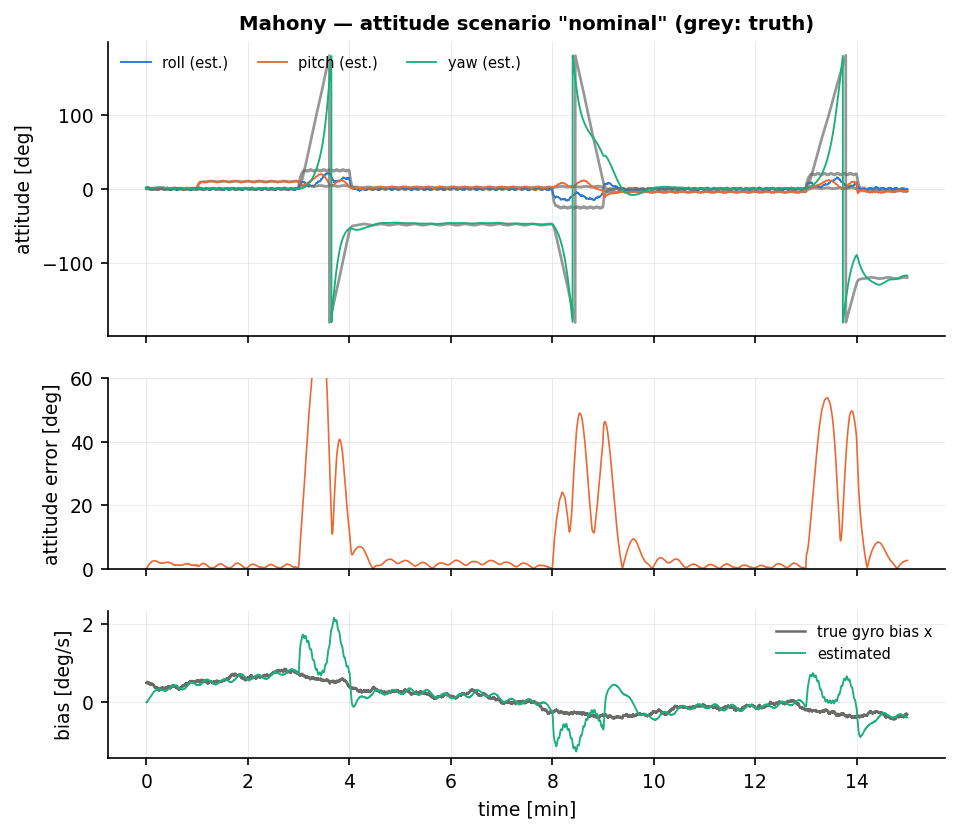
\includegraphics[width=\textwidth]{figures/imu_Mahony_nominal.png}
\caption{Mahony (published, $k_P=1$, $k_I=0.1$) on the nominal mission: the bias integrator
(bottom) is driven by the specific-force disturbance of the turns.}
\end{figure}
\begin{figure}[H]\centering
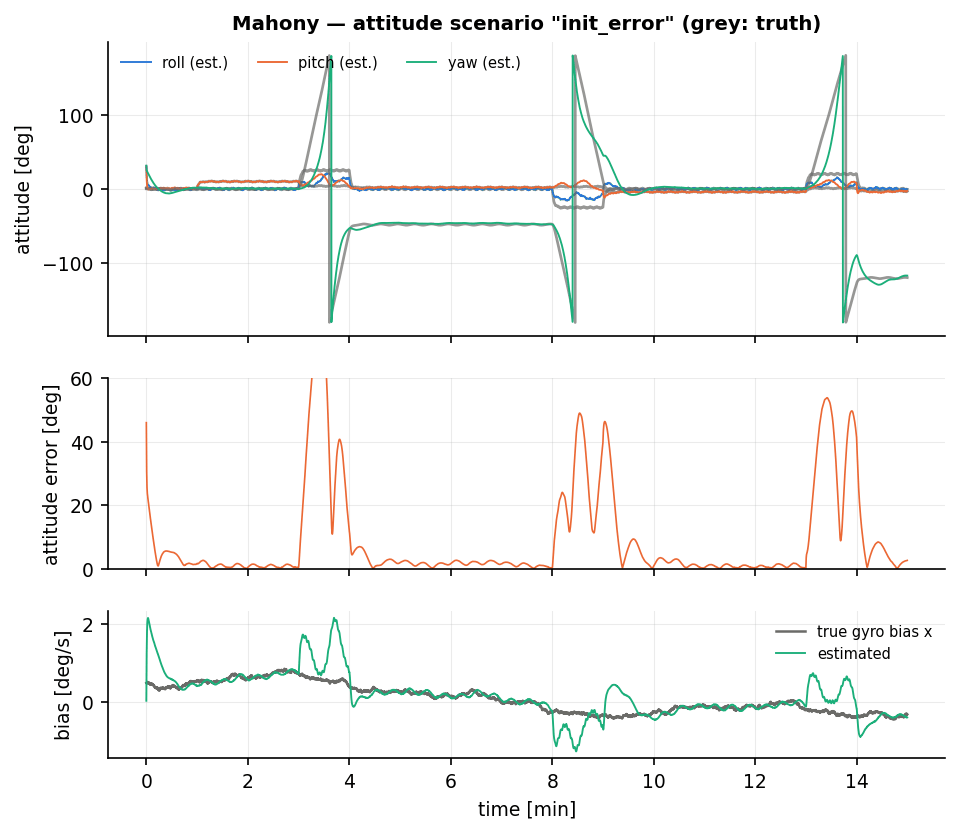
\includegraphics[width=\textwidth]{figures/imu_Mahony_init_error.png}
\caption{Mahony filter with a $46.6^\circ$ initial attitude error.}
\end{figure}

On \texttt{nominal} the published filter gives $\text{RMS}=\SI{18.40}{\degree}$ (roll $6.24$,
pitch $2.94$, yaw $\SI{17.30}{\degree}$), $\text{RMS}_{\text{ss}}=\SI{19.33}{\degree}$, peak
$\SI{76.3}{\degree}$, bias RMSE $\SI{1.24}{\degree\per\second}$, $\SI{130}{\nano\second}$/step and
312\,bytes; it is marked lost on every scenario. Per phase (seed~1),
\[
1.72\;/\;1.06\;/\;\mathbf{45.97}\;/\;2.38\;/\;\mathbf{29.98}\;/\;7.38\;/\;\mathbf{38.18}\;/\;5.46
\ \SI{}{\degree}
\]
for take-off / climb / turn\,1 / cruise / turn\,2 / descent / turn\,3 / final. In level flight it is
the best of the light filters --- $\SI{1.06}{\degree}$ in the climb, well inside the
$\SI{2}{\degree}$ convergence criterion and close to the $\SI{0.65}{\degree}$ sensor floor, because
the $\SI{3}{\second}$ loop averages part of the heading-dependent hard-iron error away --- and in
the turns it is the worst in the family, because the Lyapunov argument does exactly what it
promises. That split also explains the otherwise puzzling $t_{\text{conv}}=\SI{24}{\second}$ in the
table next to a $\SI{19.33}{\degree}$ steady-state RMS: the filter is excellent between the turns
and hopeless inside them.

Table numbers are three-seed means; the gain sweeps below are single-seed (seed~1) diagnostics.

\paragraph{Gain sensitivity.} On \texttt{nominal}, $k_P=0.5/1/2$ at $k_I=0.1$ give
$22.64/18.46/\SI{17.01}{\degree}$ with bias RMSE $1.81/1.25/\SI{0.86}{\degree\per\second}$: a faster
attitude loop leaves less of the disturbance for the integrator. The $k_I$ sweep at $k_P=1$ gives
$11.97/18.46/30.03/\SI{28.10}{\degree}$ for $k_I=0/0.1/0.2/0.3$ with bias RMSE
$0.62/1.25/2.41/\SI{2.63}{\degree\per\second}$. Setting $k_I=0$ (a pure nonlinear complementary
filter, Hamel \& Mahony~\cite{hamel2006}) gives the best \texttt{nominal} number of all,
$\SI{11.97}{\degree}$, but $\SI{20.94}{\degree}$ on \texttt{gyro\_bias} and no bias output at all ---
the integrator is being paid for in disturbance sensitivity and paid back in bias rejection.

\paragraph{Weighting and reference choices.} Reducing the magnetometer weight to $k_m=0.25$ improves
\texttt{nominal} to $\SI{15.78}{\degree}$ and \texttt{mag\_disturbance} to $\SI{18.69}{\degree}$
(from $20.44$): with the accelerometer wrong for a third of the mission, less magnetometer weight
means both less dip-amplified heading error and less exposure to the magnetic disturbance.
\code{mag\_ref\_measured} gives $\SI{22.64}{\degree}$ and \code{mag\_yaw\_only} gives
$\SI{21.76}{\degree}$: both discard the magnetometer's contribution to $\bm{M}$ in the tilt
directions, which on this mission --- where the accelerometer is the unreliable sensor --- is
exactly the wrong information to throw away.

\paragraph{Scenario behaviour.} \texttt{gyro\_bias} ($\SI{3}{\degree\per\second}$) costs almost
nothing in attitude ($\SI{18.44}{\degree}$, $t_{\text{conv}}=\SI{32}{\second}$): the integrator does
its job, and the measured bias RMSE is the same $\SI{1.28}{\degree\per\second}$ as on nominal, i.e.
the integrator tracks the extra $\SI{3}{\degree\per\second}$ and is limited by the turn disturbance,
not by the bias size. \texttt{mag\_disturbance} costs $\SI{2.0}{\degree}$ ($20.41$): with no gating,
the $\SI{25}{\micro\tesla}$ offset enters $\bm{\omega}_{\text{mes}}$ directly and the cruise-phase
RMS rises from $2.38$ to $\SI{17.36}{\degree}$ for the duration. \texttt{vibration} is free
($18.28$): the $k_P$ loop is a $\SI{3}{\second}$ low-pass and averages the extra accelerometer noise
away. \texttt{high\_dynamics} costs $\SI{0.35}{\degree}$ and is the only scenario the published
filter never converges on.

\paragraph{Initial-error transient.} From $46.6^\circ$ the filter reaches $5^\circ$ in
$\SI{8.3}{\second}$ and $1^\circ$ in $\SI{10.3}{\second}$, consistent with the $\SI{3}{\second}$
loop time constant of \eqref{eq:mh-poly} plus the bias-loop settling. From $90^\circ$ it takes
$\SI{1.3}{\second}$ to $5^\circ$ but $\SI{60.7}{\second}$ to $1^\circ$: the large-error correction
is fast (the cross product is largest near $90^\circ$) but the residual bias transient is slow.

\section{The gated variant (\texttt{Mahony-Gated})}\label{sec:mh-gated}
The second registered instance is the same filter --- same $k_P=1$, $k_I=0.1$, same known reference
directions, same Eqs.~\eqref{eq:mh-wmes}--\eqref{eq:mh-prop} --- with \code{gate = true}. This is an
\textbf{engineering addition on top of the published algorithm, not something Mahony, Hamel and
Pflimlin proposed}: the accelerometer weight $k_a$ is multiplied by the disturbance weight
\eqref{eq:cf-weight} of Chapter~\ref{ch:att-complementary}, built from the low-pass-filtered
deviation of $\norm{\bm{f}}$ from $g$ \emph{and} from the rate-driven manoeuvre bound
$V_{\text{ref}}\norm{\bm{\omega}_{yz}}$ of Chapter~\ref{ch:att-mekf},
Remark~\ref{rem:mekf-turn}; beyond a threshold the accelerometer term is dropped from
$\bm{\omega}_{\text{mes}}$ entirely. The Lyapunov argument of \eqref{eq:mh-V}--\eqref{eq:mh-Vdot}
survives the modification --- a time-varying $k_a(t)\ge0$ only changes $\bm{M}$, and
$\dot V=-k_P\norm{\bm{\omega}_{\text{mes}}}^2\le0$ still holds --- but the observability condition
$\bm{M}\succ0$ now fails whenever the accelerometer is gated out, so the guarantee degrades from
almost-global convergence to convergence \emph{while at least two independent directions are
admitted}. The extra cost is $\SI{2}{\nano\second}$/step.

\begin{remark}[Why this is safe here and not for Madgwick]
The manoeuvre detector consumes the bias-compensated rate $\bm{\omega}_y-\hat{\bm{b}}$, so it needs
a bias state to work. Mahony has one by construction, Eq.~\eqref{eq:mh-b}, and the $k_I$ loop
converges in about $\SI{20}{\second}$ --- fast enough that an uncompensated
$\SI{3}{\degree\per\second}$ offset never latches the gate. Madgwick has one only if $\zeta>0$,
which is why \texttt{Madgwick-Gated} must enable both together
(Chapter~\ref{ch:att-madgwick}, Remark~\ref{rem:mw-package}).
\end{remark}

% Copyright 2026 Sreeram Anil
% SPDX-License-Identifier: CC-BY-4.0
\begin{table}[H]\centering\footnotesize\setlength{\tabcolsep}{3.5pt}\caption{Mahony-Gated: attitude benchmark (mean over seeds; all angles in degrees; $t_\mathrm{conv}$: first time the attitude error stays below 2$^\circ$ for 30\,s; bias RMSE in deg/s; 312 bytes of state).}\label{tab:imu_MahonyGated}
\begin{tabular}{lrrrrrrrrcr}\toprule scenario & RMS & roll & pitch & yaw & max & RMS$_\mathrm{ss}$ & $t_\mathrm{conv}$ [s] & bias RMSE & lost & ns/step \\ \midrule
nominal & 2.14 & 0.62 & 0.64 & 1.94 & 8.3 & 2.03 & 24 & 0.14 & no & 132 \\
init\_error & 3.76 & 1.28 & 0.86 & 3.45 & 46.0 & 2.03 & 71 & 0.36 & no & 132 \\
gyro\_bias & 2.74 & 0.80 & 0.63 & 2.54 & 13.1 & 2.03 & 49 & 0.35 & no & 134 \\
mag\_disturbance & 2.31 & 0.66 & 0.66 & 2.10 & 8.7 & 2.03 & 24 & 0.15 & no & 132 \\
vibration & 2.47 & 0.76 & 0.76 & 2.22 & 9.8 & 2.65 & 37 & 0.15 & no & 132 \\
high\_dynamics & 4.83 & 1.55 & 1.11 & 4.41 & 16.5 & 6.07 & 259 & 0.20 & no & 130 \\
\bottomrule\end{tabular}\end{table}

\begin{figure}[H]\centering
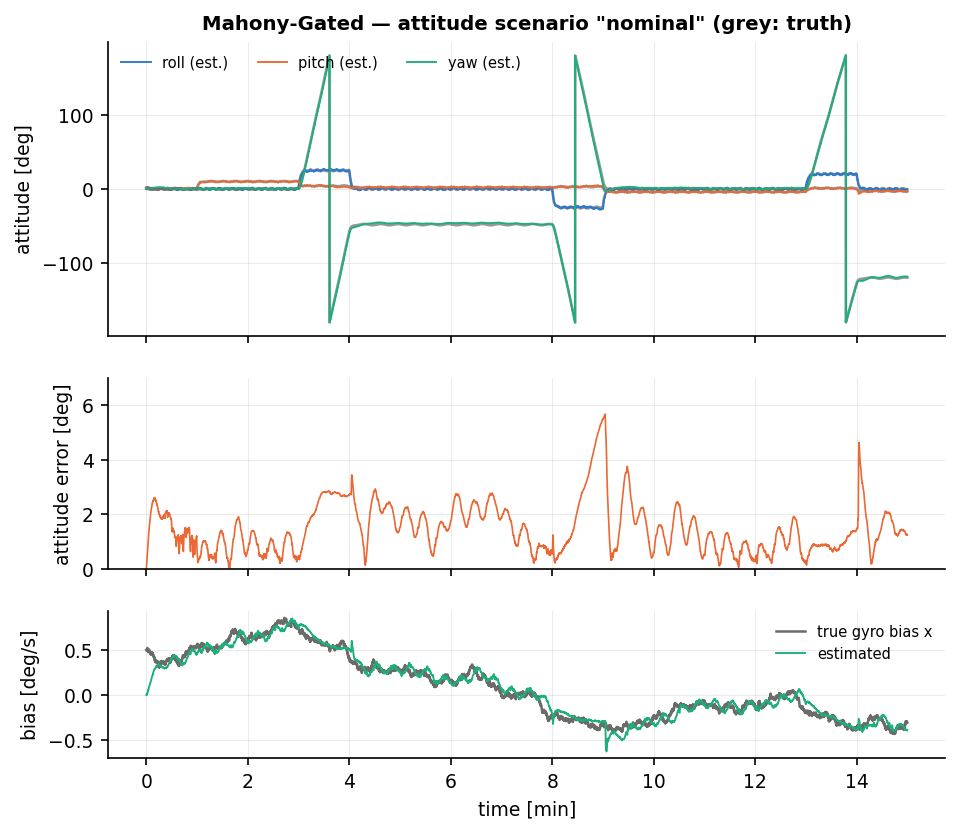
\includegraphics[width=\textwidth]{figures/imu_MahonyGated_nominal.png}
\caption{Mahony-Gated on the nominal mission: the same observer with a manoeuvre-gated
accelerometer weight. The turns are no longer visible in the error trace.}
\end{figure}

\texttt{Mahony-Gated} is the single largest improvement in this family:
$2.14/3.76/2.74/2.31/2.47/\SI{4.83}{\degree}$ across the six scenarios in table order, against
$18.40/18.51/18.44/20.41/18.28/\SI{18.75}{\degree}$ for the published filter --- a factor of
\emph{nine} on \texttt{nominal} --- with roll $0.62$, pitch $0.64$, yaw $\SI{1.94}{\degree}$, peak
error $\SI{8.3}{\degree}$ instead of $76.3$, $\text{RMS}_{\text{ss}}=\SI{2.03}{\degree}$, bias RMSE
$\SI{0.14}{\degree\per\second}$ (against a true $\SI{1.03}{\degree\per\second}$), no lost-track flag
on any scenario, and $\SI{132}{\nano\second}$/step at 312\,bytes. Per phase (seed~1),
\[
1.64\;/\;0.93\;/\;2.43\;/\;1.83\;/\;3.14\;/\;1.40\;/\;1.28\;/\;1.68\ \SI{}{\degree}
\]
--- the turns are no longer distinguishable from the cruise. It is the best estimator in the family
on \texttt{nominal} and \texttt{mag\_disturbance}, better than the MEKF ($2.48$ and $2.86$) at
\emph{one fifteenth} of the cost, and it reaches the $2^\circ$ convergence criterion at
$t=\SI{24}{\second}$.

This is the most important measurement in the chapter, and it should be read as a statement about
\emph{disturbance modelling}, not about estimator structure: the $\SI{16}{\degree}$ that separates
\texttt{Mahony} from \texttt{MEKF} in the overview table is almost entirely a difference in what the
two filters believe about the accelerometer during a coordinated turn, not in how they represent
attitude or propagate a covariance. Give the 1\,kB nonlinear observer the same belief and it matches
the $6\times6$ Kalman filter.

Three caveats, in the interest of not overselling it. \emph{(i)} On \texttt{high\_dynamics} the gated
filter degrades to $\SI{4.83}{\degree}$ --- worse, relative to its own baseline, than the MEKF's
$3.33$ --- because with tripled turbulence the gate fires often and a fixed-gain filter has no
covariance with which to re-weight what remains. \emph{(ii)} The large-initial-error transient gets
\emph{worse}: from $46.6^\circ$ the gated filter needs $\SI{16.5}{\second}$ to reach $5^\circ$
against the ungated $\SI{8.3}{\second}$, and $\SI{24.6}{\second}$ from $78.5^\circ$ against
$\SI{8.7}{\second}$, because the de-rated $k_a$ slows the attitude loop exactly when the innovation
is largest --- a fixed-gain filter cannot tell ``large residual because the state is wrong'' from
``large residual because the measurement is wrong''. This shows up in the table as
\texttt{init\_error} being its worst non-dynamic scenario ($3.76$ against $\SI{2.14}{\degree}$) and
$t_{\text{conv}}$ slipping from $24$ to $\SI{71}{\second}$. \emph{(iii)} The gate introduces two
constants ($V_{\text{ref}}$ and the editing threshold) that the published filter does not have, and
they encode an assumption about the airframe.

\section{Summary}
The Mahony filter is the right default nonlinear attitude observer: 312\,bytes,
$\SI{0.13}{\micro\second}$/step, an almost-global stability proof, and a bias state that removes the
fixed-gain filter's $b\tau$ error. Its gains are two numbers with a textbook second-order
interpretation, \eqref{eq:mh-poly}. Use it whenever the vector observations can be trusted on
average. Do not use it unmodified where they cannot: the same Lyapunov function that guarantees
convergence guarantees convergence \emph{to the disturbed solution}, which on this fixed-wing
mission costs a factor of nine in RMS and an order of magnitude in bias accuracy. Add manoeuvre
rejection --- the separately registered \texttt{Mahony-Gated} --- and it becomes, measurably,
\emph{better} than the MEKF on \texttt{nominal} and \texttt{mag\_disturbance} and within
$\SI{1.5}{\degree}$ of it on the rest, at a fifteenth of the price, at the cost of
two airframe constants and a slower large-error transient.
